
\usetikzlibrary{arrows.meta,calc,shapes,decorations.pathreplacing,patterns}
\providecommand{\computer}{%
    
\includegraphics[width=1cm]{../common/Noun_project_216.pdf}
}
\providecommand{\switch}{%
    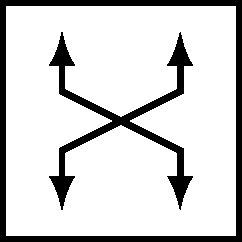
\includegraphics[width=0.9cm]{../common/fig-switch.pdf}
}
\providecommand{\router}{%
    
\includegraphics[width=0.9cm]{../common/fig-router.pdf}
}



\begin{frame}{exercise}
\begin{tikzpicture}
\tikzset{
    computer/.style={inner sep=0mm,outer sep=0mm,execute at begin node={\computer}},
    switch/.style={inner sep=0mm,outer sep=0mm,execute at begin node={\switch}},
    router/.style={inner sep=-1mm,outer sep=0mm,execute at begin node={\router},circle},
    connect/.style={draw,line width=0.5mm,Latex-Latex},
    connect big/.style={draw,line width=1mm,Latex-Latex},
}
\node[computer] (A) at (0, 2){};
\node[computer] (B) at (13, 0){};
\node[router] (r1) at (5, 0){};
\node[router] (r2) at (10, 0){};
\node[computer] (C) at (0, -2){};
\node[computer] (D) at (13, -2){};
\foreach \x/\y in {A/r1,r1/r2,r2/B,r2/D} {
    \draw[connect big] (\x) -- (\y);
}
\draw[connect] (C) -- (r1)
    node[midway,every pin/.style={arrows=-},pin={slow link}] {};
\begin{visibleenv}<2>
\foreach \x/\y in {A.east/r1.west,r1.east/r2.west,r2.east/B.west} {
    \draw[-Latex,blue,line width=.7mm] ([yshift=-3mm]\x) -- ([yshift=-3mm]\y);
}
\foreach \x/\y in {C.north east/r1.south west,r1.east/r2.west,r2/D} {
    \draw[-Latex,red,dotted,line width=.5mm] ([yshift=3mm]\x) -- ([yshift=3mm]\y);
    \draw[-Latex,violet,dashed,line width=.5mm] ([yshift=5mm]\x) -- ([yshift=5mm]\y);
}
\end{visibleenv}
\end{tikzpicture}
\begin{itemize}
\item let's say slow link has 5 MByte/s capacity, other links 20MByte/s
\item why are these fair/unfair? (by min-max fairness)
    \begin{itemize}
    \item solid = 10MByte, dotted = 2MByte/s, dashed = 3MByte/s
    \item solid = 16MByte, dashed = 2MByte/s, dashed = 2MByte/s
    \end{itemize}
\end{itemize}
\end{frame}

